\documentclass[a4paper, titlepage, oneside, 12pt]{article}%      autres choix : book  report

\usepackage[utf8]{inputenc}%           gestion des accents (source)
\usepackage[T1]{fontenc}%              gestion des accents (PDF)
\usepackage[francais]{babel}%          gestion du français
\usepackage{textcomp}%                 caractères additionnels
\usepackage{mathtools,  amssymb, amsthm}% packages de l'AMS + mathtools
\usepackage{lmodern}%                  police de caractère
\usepackage{geometry}%                 gestion des marges
\usepackage{graphicx}%                 gestion des images
\usepackage{xcolor}%                   gestion des couleurs
\usepackage{array}%                    gestion améliorée des tableaux
\usepackage{calc}%                     syntaxe naturelle pour les calculs
\usepackage{titlesec}%                 pour les sections
\usepackage{titletoc}%                 pour la table des matières
\usepackage{fancyhdr}%                 pour les en-têtes
\usepackage{titling}%                  pour le titre
\usepackage[framemethod=TikZ]{mdframed}% print frames
\usepackage[justification=centering]{caption}%                  for captionof
\usepackage{listings}%				  pour insertion de codes 
\usepackage{enumitem}%                 pour les listes numérotées
\usepackage{microtype}%                améliorations typographiques
\usepackage{csvsimple}%                convertir un fichier .csv en tableau
\usepackage{url}%					  amélioration afficahge url
\usepackage{hyperref}%                 gestion des hyperliens
\usepackage{svg}	%					  gestion des svg	
\usepackage{float}%					  gestion des figure non flotante
\usepackage{fullpage}
    
\usepackage{titling} %  				  gestion des subtitles 
\newcommand{\subtitle}[1]{%			  definition d'une nouvelle commande sous-titre
  \posttitle{%
    \par\end{center}
    \begin{center}\large#1\end{center}
    \vskip0.5em}%
}                
\lstset{language=c++}
\definecolor{codegreen}{rgb}{0,0.6,0}
\definecolor{codegray}{rgb}{0.5,0.5,0.5}
\definecolor{codepurple}{rgb}{0.58,0,0.82}
\definecolor{backcolour}{rgb}{0.95,0.95,0.92}
 
\lstdefinestyle{mystyle}{
    backgroundcolor=\color{backcolour},   
    commentstyle=\color{codegreen},
    keywordstyle=\color{magenta},
    numberstyle=\tiny\color{codegray},
    stringstyle=\color{codepurple},
    basicstyle=\footnotesize,
    breakatwhitespace=false,         
    breaklines=true,                 
    captionpos=b,                    
    keepspaces=true,                 
    numbers=left,                    
    numbersep=5pt,
    otherkeywords={uint16_t},                  
    showspaces=false,                
    showstringspaces=false,
    inputencoding=latin1,
    showtabs=false,                  
    tabsize=2
}
\lstset{style=mystyle}

\hypersetup{%
    pdfborder = {0 0 0}
}


                                    
\title{Rapport du Projet PSAR :\\ Dispositif Autonome de Synthèse Sonore}
\subtitle{Encadrant : Hugues Genevois}

\author{Pierre Mahé}
\date{4 mai 2015}

\begin{document}  
 \begin{figure}[b]
	\includegraphics[width=120px] {upmc_logo.jpg}
	\hspace{7cm}
	\vspace{-2cm}
	\includegraphics[width=120px] {LogoLAM.jpg}
\end{figure}

\maketitle 
\tableofcontents

\newpage
\section{Introduction}
\subsection{Contexte Global}

\paragraph{}
Le projet DASS, Dispositif Autonome de Synthèse Sonore, est une collaboration de Michel RISSE, compositeur de "Décor Sonore" ayant à son actif de nombreuses créations et dispositif sonores, et de Hugues GENEVOIS, chercheur au LAM de L'Institut Jean le Rond d'Alembert.

\paragraph{}
Le projet consiste à mettre en place un dispositif générant du son en prennent en compte sont environnement dans le but de souligner les sons près-existant dans cet environnement. Le dispositif recueille les informations à l'aide de capteurs diverses permettant de récupérer les bruits ambiants, la luminosité, la température...

Dans un première temps, le dispositif devrait être la base pour une installation artistique, se déroulant en juillet prochain, dans le cadre d'un festival de musique de Noirlac. Dans un second temps Hugues GENEVOIS et Michel RISSE voudraient réaliser une installation plus importante avec de nombreux dispositifs, avec pour chacun d'eux des comportements et des caractéristiques propre. Dans le but de voir l’interaction qu'ils pourraient avoir ensemble et les comportements qui en émergeraient.

\subsection{Objectifs du PSAR}
\paragraph{}
Dans le cadre de mon projet PSAR, mon but était de créer un premier prototype du dispositif pour s'en service comme base par la suite.\\
J'avais donc pour mission de créer un dispositif portable interagissant avec son environnement. Ce dispositif doit capter l'environnement à l'aide de capteurs : micro, luminosité, température, et humidité. Il devra traiter ces données pour en extraire des informations pertinente sur les changements se produisant autour de lui (chants d'oiseaux, passage d'une personne au alentour...). Grâce à ces informations, il devra synthétiser du son.
\paragraph{}
La synthèse devra être paramétrable, pour permettre au compositeur de modifier
l’influence des différents capteurs sur la synthèse sonore.\\
De plus une interface utilisateur devra être présente permettant au compositeur de simuler des données captés. Cela lui permettra de faire des expérimentations de sa composition.
\paragraph{}
Dans l’optique de la reproduction de ce dispositif pour des installations plus important. Une procédure devra permettre à un utilisateur de pouvoir reproduire l’ensemble du système, aussi bien niveau matériel que logiciel.
\paragraph{}
Le dispositif devant être portable, le programme doit fonctionner sur une nano-ordinateur de type \texttt{Udoo Quad}. De plus le langage du programme principal doit être le Pure Data, pour assurer une maintenabilité et une extensionnalité plus facile.
\subsection{La Carte Udoo}
\begin{figure}
  \centering
  \includegraphics[width=300px]{udoo.jpg}
  \caption{Carte Udoo}
\end{figure}

\paragraph{}
La carte Udoo est un nano-ordinateur embarquant un processeur ARM et la connectique d'un ordinateur classique avec une entrée et sortie micro, des sortie USB, HDMI, carte WIFI... L'entrée et la sortie audio étant d'une qualité suffisante pour notre projet, il ne sera pas nécessaire ajouter à la Carte Udoo une carte son externe.\\
La caractéristique de cette carte est d’être compatible Arduino et d'offrir les mêmes connectiques (GPIO, SPI ...) qu'une Arduino Mega ce qui permet de simplifier la réception des capteurs de plus il permet d'utiliser les bibliothèques déjà implémenté par la vaste communauté Arduino.\\
Pour stocker les données, la carte utilise une carte micro SD, ce qui est également un avantage pour le projet car cela permet de dupliquer la partie software du dispositif avec une simple copie de carte mémoire.\\
Le système d'exploitation installé est un version légère d'Ubuntu, permettant d'utiliser l’environnement Linux.

\subsection{Pure Data}
\subsubsection{Présentation générale}
\begin{figure}
  \centering
  \includegraphics[width=200px]{pd.jpg}
  \caption{Patch Pure Data}
\end{figure}
\paragraph{}
Pure Data (\texttt{Pd}) est un logiciel, open source, de programmation graphique pour la création et l’interaction musicale et multimédia en temps réel. Il permet également de gérer des flux entrants dans l'ordinateur (données de périphériques ou événements réseau par exemple) et de gérer des flux sortants (par des protocoles de réseau ou protocoles électroniques pour le pilotage de matériels divers).\\
Pure Data est un système module où il est possible de définir des sous-modules qu'il est possible de ré-utiliser à sa guise dans d'autre programme appelé \texttt{patch}.\\
En Pure Data tous les objets (modules ou données) sont des \texttt{boites}.
Ce langage est un langage très faiblement typé. Il existe quatre types de données:\\
\begin{itemize}
\item \textbf{Les Nombres}, qui peuvent représenter des nombres entiers comme des nombres à virgules.
\item \textbf{Les Message}, qui sont des messages strictement textuels.
\item \textbf{Les Symboles}, qui corresponde aux messages mixtes, caractère, chiffres...
\item \textbf{Les Tableaux}, qui sont uniquement des tableaux de nombres.
\end{itemize}
Il existe d'autres types de données comme les listes qui même si leurs représentation interne différant des messages ou des symboles sont graphiquement identique à un message (avec comme premier mot \texttt{list}). De plus pour changer une liste en message, il suffit de supprimer le mot clé \texttt{list}.\\
Une boite Pure Data à une ou plusieurs entrées et une ou plusieurs sortie, toutes les entrées et sorties peuvent recevoir et envoyer n'importe quel message. On peut connecter deux modules en reliant la sortie de l'une avec l'entrée de l'autre.


\paragraph{}
Le Pure Data étant un logiciel orienter interaction, il est possible à tous moment de modifier son patch en ajoutant des boites au cours de l’exécution du programme, il n'est pas nécessaire de relancer le programme. Cela peut permet de modifier le patch en direct sans avoir l’interruption dans le flux audio sortant.

\paragraph{}
Pure Data a aussi l'avant d'être facilement documentable car il est possible d'associer à une boite, une boite d'aide avec une explication et des exemples minimal.\\
Cela s’avère très utile pour la compréhension de certaines boites complexes et permet de bien dissocier code et documentation.
\paragraph{}
Un autre atout de Pd est le nombre de d'outils déjà implémenté dans le logiciel et les boites créé par la communauté. Certaine procéder à des traitements complexes, comme la détection en temps réel de fréquence ou le filtrage performant, lecture de fichier musicaux...

\subsubsection{Externals}
\paragraph{}
En Pure Data, le stockage de donnée est asses complexes c'est pour cela que pour procéder à des algorithmes complexes, il est possible d'avoir recours à des\texttt{Externals}.\\
Les externals sont des boites programmées en \texttt{c++}. 

\paragraph{}
Il existe plusieurs API pour programmer des externals. Dans ce projet nous avons choisi d'utiliser \texttt{Flext} pour sa simplicité d'utilisation. De plus cette API est développé par Thomas GRILL, un des principal contributeurs de Pure Data ce qui garantie une parfaite compatibilité avec Pd et une certaine assurance que l’outil reste longtemps maintenu. \\
La communauté des développeurs Pure Data étant limitée (une dizaine de personne au total), cela a sont importance car malheureusement beaucoup d'outils ne sont pas maintenus suffisant ou ne sont plus complètement compatible avec Pure Data.  

\subsection{Structure du projet}
\paragraph{}
Nous avons décidé de diviser le programme en cinq modules:
\begin{figure}[H]
  \centering
  \includegraphics[width=400px]{structprojet.jpg}
  \caption{Structure du projet}
\end{figure}

\paragraph{}
La partie acquisition des données des capteurs se fera par le biais de la communication entre la partie Arduino et Pure Data.\\
Nous avons écrit un programme Arduino qui va envoyer périodiquement les valeurs des différents capteurs au programme Pd.

Informations collectés par la partie Arduino:
\begin{itemize}
\item Luminosité
\item Température
\item Humidité
\end{itemize}

\paragraph{}
La seconde partie de l'acquisition est la réception du signal sonore, que l'on doit traiter pour pouvoir en extraire des informations pertinentes.\\
Le son capté par le micro est pollué par des sons ambiant, typiquement le bruit d'une route proche ou d'une machine bruyante. Ces bruits sont généralement continu, grave (moins  de 100 hertz) donc très énergétique. Ils peuvent donc fausser les résultats  et alourdir les traitements en aval.\\
Les bruits naturels de cette fréquence sont très rare. De plus musicalement ces bruits sont asses pauvres.\\
Pour toute ces raisons il est préférable de les atténuants en utilisant des filtres.\\
Pour les mêmes raisons, nous avons filtré pour éliminer les fréquences au dessus de 6000 Hertz.


\paragraph{}
Dans la partie extraction, avec le compositeur et le chercheur nous nous sommes questionné sur les informations pertinentes à extraire pour la composition musicale.\\ 
En prenant en compte le fait que la carte à une capacité de calcul limité, cela ne permet pas de faire tous les traitements coûteux en temps de calcul.

\paragraph{}
La composition musicale est la partie propre au compositeur, et correspond réellement à la partie création artistique. Plus que la fabrication de ce module, la question a été :  comment permettre au compositeur de la créer et de pouvoir la modifier le module dans le dispositif à distance, sans avoir besoin  de brancher un écran ou un clavier.

\paragraph{}
Il y plusieurs techniques de synthèses musicales. Certaines sont plus complexes et gourmands en ressources.\\ Nous avons choisi une synthèse simple. La synthèse étant très lié à la partie création musicale, le module de création musical étant rudimentaire, il en est donc disproportionné de faire un module de synthèse très complexe. 

\paragraph{}
En plus de cette structure installé dans le dispositif, une interface graphique a été crée, elle communique à distante avec le dispositif.\\
L'utilisateur peut envoyé des données pour remplacer les informations reçu des capteurs, il peut de également changer la partie création musicale.

\section{Récupération de l'environnement}
\paragraph{}
L'un des avantages de la carte Udoo est d'être compatible Arduino est donc de proposer les mêmes connectiques qu'une Arduino Mega. Cela permet d'utiliser le même langage, d'utiliser les bibliothèques déjà écrites ainsi que les mêmes capteurs.\\
De plus la partie  micro contrôleur étant connecté directement à la partie ordinateur via un bus spécial. La vitesse de communication est plus rapide et la latence est plus courte par rapport à une connexion USB classique.

\paragraph{}
Dans les informations que peuvent envoyés un capteur deux choses sont intéressante, la première la valeur absolu et la variation de celle-ci (si elle augmente ou si elle diminue).
\subsection{Dispositif et capteurs}
\begin{figure}
	\centering
	\includegraphics[width=200px]{montage.jpg}
		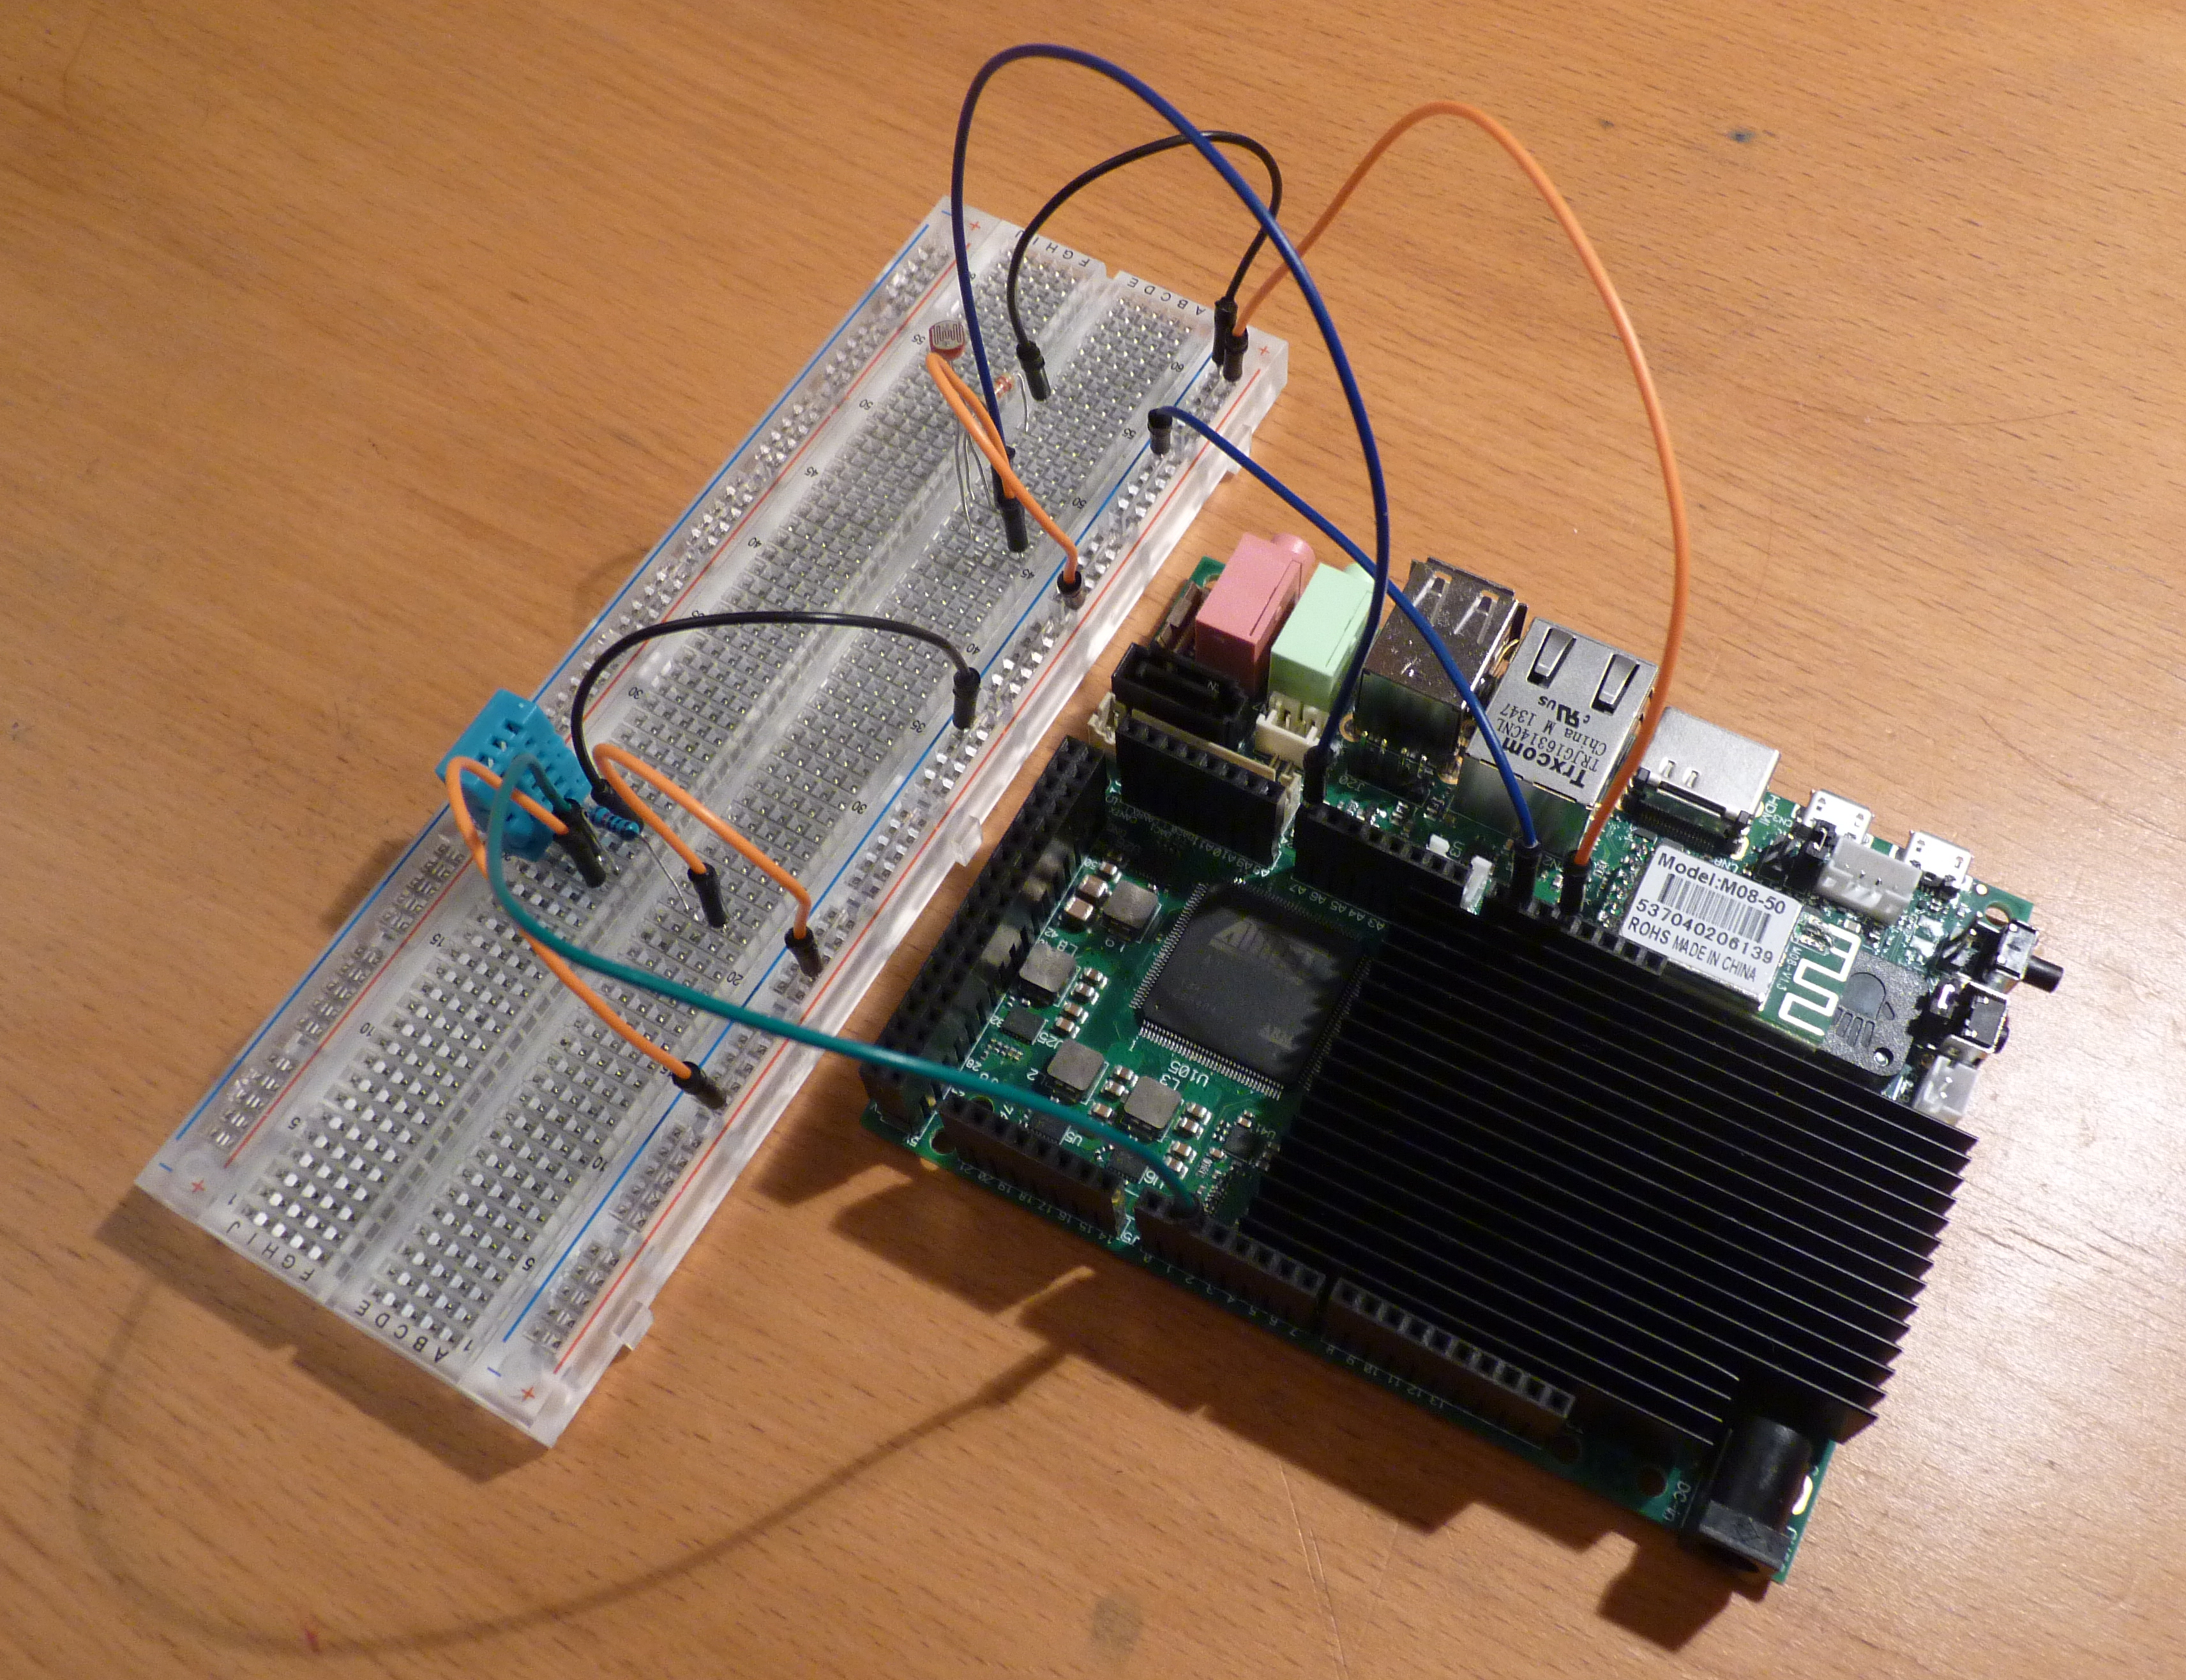
\includegraphics[width=200px]{montagephoto.jpg}
	\caption{Montage du dispositif}
\end{figure}
\paragraph{}
Dans le cadre du projet, seul trois capteurs étaient prévu mais le programme permet un ajout de capteurs aisé.\\
Les capteurs utilisés sont des capteurs basique: un capteur de luminosité, de température et d'humidité.\\

Pour capteur la luminosité, nous avons utilisé une photo-résistance, son fonctionnement est asses simple, plus la luminosité va être forte plus la résistance interne de composant est faible. \\
Il suffit donc de récupérer la tension au borne de composant pour connaître l'indice de luminosité.\\ 
Malheureusement cette indice ne permet pas de connaître l'intensité lumineuse en Candela ou en Lux mais permet d'avoir une échelle relative de valeurs. Cela est suffisant dans le cadre du projet.
\paragraph{}
Pour la température et l'humidité la récupération la valeur est très similaire. Par contre, contrairement à la luminosité grâce à une formule (dépendant de chaque capteur) il est possible d'avoir la température ou l'hygrométrie précise (degrés Celsius et en pourcentage). 

\subsection{Communication inter plate-forme}
\paragraph{}
Pour la partie micro-contrôleur l'envoi de données est asses intuitive car il suffit d’écrire sur le port Série (\texttt{Serial port}), grâce à des fonctions implémenté de base en Arduino.\\
Pour la partie ordinateur avec le logiciel Pure Data, il faut utiliser une boite pour se connecter au périphérique puis il est possible de lire et écrire sur celui.\\
La connexion entre l'Arduino et Pure Data devant être unique, il a fallu trouver un moyen de pouvoir différencier les données des différant capteurs. 

\paragraph{}
Pour communiquer entre les deux parties, un micro-protocole à donc était défini pour étiquette les données envoyés.\\
À intervalle régulier (toutes les seconds) le programme Arduino lit les valeurs des capteurs et les envoi un message de la forme :
\begin{lstlisting}
NOM_CAPTEURvl: VALEUR;		//vl pour la valeur
MON_CAPTEURvr: VALEUR;		//vr pour la variation
\end{lstlisting}

Pour ajouter un capteur, il suffit d'écrire un nom de capteur -pas encore utiliser- et de modifier le programme Pure Data pour traiter la nouvelle étiquette.

\paragraph{}
Dans un second temps, il s'est avère utile de pouvoir changer, au cours de l’exécution, le délai entre chaque envoi de valeurs. \\
Pour cela il a fallu permettre à l'Arduino de pouvoir recevoir des données. Les messages ayant la même forme que l'envoi de données avec l'étiquette \texttt{delay}.\\
Ce moment là, nous avons découvert un défaut de Pure Data. Étant un langage très faiblement typé. Les données reçu de l'Arduino sont des octets que Pure Data caste en type Nombre et il n'existe pas d'objet permettant à partir de ce flux d'octets de récupérer des \texttt{integers} (valeur des capteurs envoyé par la partie Arduino).\\

\paragraph{}
Au première abord nous avons voulu utiliser l'objet \texttt{PakcOSC} qui permet de convertir un message quelconque en commande OSC (\texttt{Open Sound Control}). Ce protocole étant un protocole utilisant le codage ascii, il serait possible de l'utiliser pour encoder et décoder les communications avec l'Arduino. \\
Mais cela aurai été une manipulation de l'objet de base de plus cela pourrai porter à confusion, le dispositif ne gérant en rien le protocole.\\
Nous avons discuté avec Hugues GENEVOIS et la programmation d'un externals apparaît comme plus adapté.

\subsection{External pour la communication}
\paragraph{}
En s'inspirant du fonctionnement des objets \texttt{PackOSC} et \texttt{UnPackOSC}, nous avons programmé deux externals : Un qui reçois un message et le transforme en tableau d’octets (en code ascii plus exactement) en ajoutant le code ascii d'un point virgule à la fin pour délimiter le message.\\
Le second reçois un flux d'octets et le stocke dans un tableau jusqu’à recevoir un point virgule, à ce moment là il envoi toute la chaîne reçue.\\
Le fait d'utiliser le caractère ';' n'est pas un problème car en Pure Data ce caractère est généralement le délimiteur interne pour indiquer la fin de chaîne, de liste et de tableau, d'une lecture fichier ainsi que la fin des messages TCP.

\section{Traitement audio}
\subsection{Acquisition audio}
\paragraph{}
Comme nous l'avons dit dans l'introduction du projet, Nous avons filtré le signal audio capté par le micro pour supprimer les bases fréquences et les hauts fréquences.\\
Nous avons chercher à savoir déterminer les fréquences de coupure à partir des quelles il n'y a plus d'informations pertinentes. Nous nous sommes rendu compte qu'au dessus de 6000 Hertz il n'y avait plus de son avec une fondamentale à cette haute, le signal capté ne sont plus que des harmoniques de sons plus grave.\\ %TODO (Voir l'annexe rappel musical pour les explications sur les fondamentales et les harmoniques).\\
Pour les sons très graves, il n'existe pas de sons produits par la nature à des fréquences inférieurs à 100 Hertz. Nous avons donc ajouté un filtre à notre module d'acquisition pour pouvoir supprimer les fréquence qui sont des bruits parasites.

\subsection{Traitement du son bas niveau}
\subsubsection{Filtrage}
\paragraph{}
Une information qui paraissait essentiel à extraire était les notes et les mélodies qui sont joué dans l’environnement.\\
Il est asses facile de déterminer la fréquence principal d'un signal, il suffit de prendre la forme générale du signal. Il existe plusieurs boites en Pd pour le faire tel que \texttt{Fiddle\~} ou \texttt{Signum\~}.\\
Contrairement au suivis simple la détection de notes joué simultanément ou le suivi de  plusieurs de mélodies simultanément est très difficile et fait encore partie l'objet de recherche.\\
Il n'est pas possible de déterminer toute les notes joués dans le monde fréquentiel, il est nécessaire de passe dans le monde spectral en utilisant la Transformé de Fourrier. Il existe une boite en Pure Data \texttt{FFT}. La boite manquant de possibilité de paramétrage (nombre de points...).
\begin{figure}[H]
	\centering
	\includegraphics[width=300px]{fft.jpg}
	\caption{Transformée de Fourrier}
\end{figure}
\paragraph{}
Nous avons implémenté un programme en \texttt{C} pour pour faire une transformée Fourrier Rapide (\texttt{FFTW}) dans l'optique d'en faire une boite pour l'utiliser dans Pure Data.
Ce qui permettrait de pouvoir mieux paramètre la transformation.\\

Apres test notre programme était aussi trop gourmand pour la carte. Malgré le fait que la complexité de la FFT est de N*log(N). Mais le N correspond au taux d’échantillonnage du signal (le nombre de point du signal). Notre signal est échantillonné à 44 kHertz il y a donc 44100 points à traiter par seconde ce qui est lourd pour la carte (si nous voulons pouvoir faire d'autres traitements en parallèle).

\paragraph{}
Après ces tests insatisfaisante, nous nous sommes orienté dans une autres directions, Hugues GENEVOIS nous a conseillé de partager le spectre sonore en plusieurs bandes de fréquences à l'aide de filtres passe-bande et de suivre de détecter la fréquence principale (la plus forte) de chaque bande, avec un \texttt{fiddle\~}.\\
Après avoir implémenté ce mécanisme en Pure Data, un nouveau problème est apparu. Les filtres ne coupant pas parfaitement les fréquences en dehors de leur bande, les objets \texttt{fiddle\~} détecte parfois des fréquences principale n’appartenant pas à leurs bande de fréquence. Il y avait donc plusieurs filtres qui détectait la même fréquence se qui était asses problématique.\\
Ce phénomène arrive fréquemment quand le son enregistré contenait peu de fréquence (voir une seule). Les filtres qui n’étaient pas centrés sur la fréquence capté par le micro avait peu de signal dans leurs bande et par conséquent avoir tendance à récupérer les résidus, et donc la fréquence en dehors de sa bande de fréquence.
\begin{figure}[H]
	\centering
	\includegraphics[width=300px]{filtre.jpg}
	\caption{Bandes de Fréquences}
\end{figure}
\paragraph{}
Pour résoudre ce second problème, nous avons utilisé des \texttt{Noise Gates}.\\
Une \texttt{Noise Gate} est un élément trés utiliser en musique, il correspond à une boite ne laissant passer que le signal sonore au dessus d'une certaine intensité. Si le signal est trop faible le signal en sortie de la boite est égale à zeros.
Cela permet quand il n'y a pas de fréquence centré sur le bande de fréquence de supprimer les sons venant des autres bandes de fréquences. Étant atténuer par les filtres, ces sons ne passent pas la \texttt{Noise Gate}, ce qui limite le problème de la détection de fréquence erroné.\\
L’Élément clé pour limiter les erreurs est donc le seuil à partir duquel la \texttt{Noise Gate} laisse passer le signal.\\ Si il est trop faible, il restera beaucoup de fausses détections. Si le seuil est trop élevé, on va avoir tendance à ne pas détecter des fréquences pourtant très proche de la bande passante.

\subsubsection{Détecteur de notes}
\paragraph{}
Ce dispositif produit beaucoup moins d'erreurs que les précédents mais il n'était pas satisfaisant pour pouvoir faire un suivi de mélodie s'étalant sur plusieurs bandes de fréquences. Cela se traduise par la détection de morceaux de mélodie haché.
\paragraph{}
Nous avons donc décidé d'abandonner l'idée de suivre plusieurs mélodies simultanément et de ne garde que la mélodie principal du signal. \\
Et de n’utiliser les notes récupérer à la sortir des les filtres uniquement pour connaître les notes présentes.\\
Cette information peut semblé peu pertinente mais il est très important pour le dispositif de savoir quelles notes sont joué, si la mélodie qu'il capte utilise uniquement deux notes, il serait très dissonant que le dispositif joue une troisième note qui n'a rien a voir avec les deux premières.\\ Cela donnerai un rôle trop importante est donc contradictoire avec le projet initial qui était de faire un dispositif m’étant en valeur l’environnement.\\
Dans ce but, un compteur de notes a était implémenté. Il collecte les notes reconnues à la sortie des filtres et à intervalle régulier le compteur va nous donner la fréquence d’apparitions des notes.\\
Pour ne pas faire de dissonance il suffira au module de synthèse de piocher des notes tirés au hasard dans les notes les plus fréquemment joués.\\
Il est également possible d'imaginer une synthèse qui regarderait les notes joués pour jouer des notes pour compléter les accords.

\subsubsection{Bandes de fréquences}
\paragraph{}
Avec ce système de détection de note, ils est possible de savoir la fréquence d'apparition des notes mais il n'est pas possible de savoir la hauteur des sons captés.\\
Nous avons donc ajouter un module pour mesurer l'amplitude du signal sur chaque bande de fréquence pour savoir comment sont reparti les notes sur les bandes de fréquences, si les bruits captés par le micro sont plutôt aiguë ou grave.

\subsection{Traitement du son haut niveau - Extraction des méta-données}
\subsubsection{Mélodie et rythme}
\paragraph{}
Comme expliqué dans la section précédente, nous avons implémenté un module pour détecter la mélodie principal du signal.\\

Il était naturel d'implémenter un module homologue à la détection de note, mais là pour déterminer les rythmes.\\
Pour synthétiser des sons avec des rythmes proches des sons environnent.\\
Concrètement si une personne marche prés du dispositif, il pourrait répondre en jouer des sons avec le même rythme ou dans le cas ou le il capte un chant d'oiseau, il peut réponse en jouant des notes avec le même rythme.\\

\paragraph{}
Après en avoir discuté avec notre encadrant, il nous est apparu que la meilleur méthode pour détecter un début de note est d’essayer de détecter les impacts dans un signal audio. Généralement caractéristique d'un début de note. Pour cela  nous avons calculé l’énergie du signal %TODO ANNEXE
. Puis de regarder son évolution, si une augmentation brusque apparaît (un pente supérieur à un certain seuil), cela induit la présence d'un impact et donc du début de note.\\
Pour raffiner la détection d'impact, Le module a un seuil minimal et maximal à dépasser pour considérer que l’événement est bien un début de note.
\begin{figure}[H]
	\centering
	\includegraphics[width=300px]{bonk.jpg}
	\caption{Détection de début de note.En rouge les seuils min et max\\Les flèches  représentes les notes détectés}
\end{figure}
 
\paragraph{}
Dans l’environnement les bruits sont intermittent, il est donc intéressant de grouper les événements rythmique en sequence. \\
Une sequence commence quand le dispositif détecte le début d'une note et termine après une laps de temps sans impacte (de quelques secondes).\\
Pour éviter de faire des séquences trop longue, dans le cas d'un environnement très bruyant, nous avons décider arbitrairement de limiter un nombre d’événement maximum dans une sequence (de l'ordre de la centaine).

\paragraph{}
Pour permettre au dispositif de jouer la même structure rythmique mais à différente vitesse. Le module procède à une normalisation de la duré des rythmes.\\
Le premier intervalle entre deux notes sera la référence pour toute la sequence, elle aura une valeur '1'. Tous les autres intervalles seront des multiples de cette valeurs.\\
Avec ce systèmes, il est possible de mesurer des divisions de la valeur de référence jusqu'à la quadruple croche (1/16) ce qui apparaît comme une  precision suffisante pour le dispositif.\\
Une tolérance est appliqué au calcule des durées des rythmes pour permettre une certaine approximation des rythmes. Jouer rigoureusement  plusieurs notes parfaitement égales étant quasiment impossible.\\
Les séquences détecté sont au final de la forme:\\
\begin{figure}[H]
	\centering
	\includegraphics[width=200px] {rythme.jpg}
	\caption{ Séquence Rythmique détecté}
	\includegraphics[width=300px]{structurerythme.jpg}
	\caption{Deux rythmes pouvant produire la séquence.}
\end{figure}

\subsubsection{Détection de Motif minimal}
\paragraph{}
Nous avons beaucoup discuter de la détection mélodie et rythmique avec Hugues GENEVOIS, et nous en avons tiré la conclusion qui serai intéressant d'extraire des séquences rythmes, les motifs rythmiques récupérant dans ce sequence.\\
Cette opération s’avérant complexe et peu essayé en Pure Data à cause de la difficulté de stocker et parcourir des données. La détection de motif en utilisant des externals était bien plus facile. Deux externals ont était implémenté, un pour détecter les motifs mélodies et un pour les motifs rythmique.\\
Le fonctionnement des externas étant très proche, nous n'allons ici nous limiter à la description du détecteur de motif rythmique, l'autre external fonctionnant de manière homologue.\\
L'external prend en paramètre le nombre minimal de note le motif doit être constitué au minimum.\\
La séquence rythmique est envoyé a la volé, valeur par valeur dès que le module de détection rythmique détecte un nouveau intervalle.\\
Il stock la valeur à chaque réception et va tester si il n'a pas déjà rencontre un motif contenant cette intervalle. Des qu'un motif est détecté, l'external va envoyer ce motif rythmique pour qu'il soit utilisé pour la synthèse.\\
A chaque fin de sequence, les valeurs stockés dans l'external sont supprimé, pour accueillir les valeurs de la nouvelle sequence et trouvé un autre motif.\\
Ce module ne permet pas de faire reconnaître la plus long des motifs rythmiques présent dans la sequence mais par soucis  de faire interagir rapidement le dispositif avec son environnement, il est préférable de récupérer le motif le plus vite possible même si celui ci n'est pas le plus long. Pour être sur d'avoir le plus grand motif obligerai à attendre la fin de sequence et donc à commencer a faire interagir le dispositif qu'après que l'émetteur ai fini de jouer.
\begin{figure}[H]
	\centering
	\includegraphics[width=350px]{motifrythme.jpg}
	\caption{En rouge le motif minimal. En bleu le motif le plus long de la sequence}
\end{figure}
\section{Synthèse musical}
\subsection{Synthèse du dispositif à long terme - Modèle physique}
\paragraph{}
La synthèse par modélisation physique consiste à produire des sons à partir d'un modèle informatique décrivant les propriétés physiques d'objets virtuels.\\
On donne les caractéristiques physiques (dimension, densité, élasticité...) de l'objet que l'on veut simuler, et les caractéristiques de objet qui sera l’excitateur.\\
Puis nous utilisons cette simulation d'instrument pour produire du son. Cela permet d'avoir une timbre de sons très riches et variés.\\
L'utilisateur de cette synthèse a été évoqué mais ça complexité plus élevé et son développement plus long, nous a fait préférer l'utilisation dans ce projet, d'une synthèse plus basique.

\subsection{Synthèse implémenté}
\paragraph{}
Pour ce projet, nous avons procédé à un implémentation d'un synthèse hybride utilisant la synthèse additive et soustractive pour générer du son.
\paragraph{}
La synthèse additive consiste a produire un signal audio complexe en additionnent plusieurs signaux élémentaires (typiquement des ondes sinusoïdal).
\paragraph{}
La synthèse soustractive quand à elle consiste à produire un signal audio en filtrant certaine de fréquence de signaux riche en harmoniques comme le signal carré, triangle ou dent de scie... 

\section{Interface Utilisateur}
\subsection{Première idée d’implémentation}
\paragraph{}
Le paramétrage du dispositif se faisant à distance, les données sont envoyé au dispositif par \texttt{wifi}, la carte Udoo en étant équipé.\\
Comme l'interface graphie et le dispositif communiquaient par \texttt{wifi}, Il était intéressant de permettre à l'utilisateur de s'abstraire de la contrainte d'avoir Pure Data sur l'ordinateur configurant le dispositif. \\
Dans l'optique d'une interface portable et simple d'installation, nous avions pensé la faire en Java.
\paragraph{}
En Pure Data, les communications se fait à l'aide d'une boite du nom de \texttt{netsend} qui permet d'envoyer des messages (Pd) commencent par \texttt{send}. En \texttt{Tcp} ou en \texttt{Udp} selon les paramètres de la boite.\\
\texttt{netreceiver} la boite complémentaire de \texttt{netsend}, stock les données reçus jusqu’à recevoir la fin du message, et l'envoie sur sa sortie.\\
Dans un premier temps il nous a donc fallu trouver comment Pure Data convertissait les messages avant de les envoyer si il s’agissait d'une conversion en ASCII ou un autre  mécanisme plus complexe. De plus il a fallu trouvé le caractère ajouter au message par \texttt{netsend} pour que   \texttt{netreceiver} puisse connaître la fin du message.\\
Après plusieurs expérimentations nous avons découvert que le caractère délimiteur était  le ';', ce qui nous a permit d'envoyer des messages extérieur (d'une programme Java) à Pure Data.

\paragraph{}
Après quelques testes, nous nous sommes rendu compte que le paramétrage du dispositif ne pouvait pas se faire sans connaissances en Pure Data. Par consequant, nous avons décider de change d'idée et de créer une interface graphique en Pure Data, l'utilisateur serait plus à l'aise avec une interface fait dans un langage qu'il connaît et qui à les mêmes principe et philosophie que le programme embarqué dans le dispositif. L'utilisateur pouvant également l’adapter selon ses besoins.

\begin{figure}[H]
	\centering
	\includegraphics[width=250px] {GUI.jpg}
	\caption{Interface Graphique}
\end{figure}
\subsection{Envoie des données des capteurs}
\paragraph{}
Nous avons rencontré plusieurs fois le compositeur pour savoir ce qui lui serait le plus facile et intuitif pour l'envoi de données. Il lui à paru intéressant de dessiner des courbes pour chaque capteurs, pour visualiser exactement se qui est envoyé au dispositif. Il a pense également demandé de pouvoir changer l'échelle des courbes pour pouvoir simuler de grande variations comme des très petites.\\

\paragraph{fonctionnement}
L'utilisateur peut dessiner les courbes qui désir pour chaques capteurs, quand il a fini, il se connecte au dispositif à ce moment l'interface envoie les données au dispositif qui va les stocker et tant que la connexion ne sera pas rompu par l'utilisateur, (envoi du message de déconnexion). Le dispositif va lire ces données en boucle. Chaque lecture étant espacé d'un certain délais (fixé a 100 milliseconde). Et va les substituer aux données reçu par les capteurs.\\
Pour envoyer de nouvelles données, il suffira à l'utilisateur de tracer de nouvelles courbes, de se déconnecter et de se reconnecte pour que l'envoie des données est lieux de nouveau.

\begin{figure}[H]
	\centering
	\includegraphics[width=250px] {senddata.jpg}
	\caption{Message envoyé par l'interface au dispositif}
\end{figure}

\paragraph{}
Le nombre d’échantillon envoyé à chaque fois est fixe dans le patch, elle est fixé à 256 mais il est possible de modifier ça taille en changeant les propriétés tableaux contenant les courbes de l'interface utiliser ainsi que le programme embarqué dans le dispositif.
\paragraph{}
Pour savoir à quoi correspond chaque liste de données envoyé, le premier mot en début de liste correspond au capteur (tempe pour la température, humid pour l'humidité ...). 


\subsection{Envoie d'objet Pure data}
\paragraph{}
En Pure Data, il est impossible de modifier un patch autrement que par l'interface du logiciel en ajoutant des boites ou des connections. La création du module "Création Musicale" générique, que l'utilisateur pourrait modeler à sa guise serait impossible. La création d'une nouveau module est donc obligatoire pour chaque événement différant.
\paragraph{}
Nous nous sommes questionné sur comment  pouvoir changer la partie "Création musicale" à distance.\\
La première idée envisage a était de faire un script \texttt{Bash} pour envoyer un patch programmé sur l'ordinateur de l'utilisateur vers le dispositif.\\
Le défaut majeur de cette technique est que cela force l'utilisateur à connaître les base du  \texttt{Bash} et les commandes utile pour maintenir le script. \\
Ce qui peut paraître évident pour une personne travaillant dans le domaine de l'informatique mais qui est rare chez les utilisateurs de Pure Data, utilisant un langage graphique pour s'abstraire du code informatique. De plus cela  oblige à utiliser un autre outil que Pd.

\paragraph{}
Nous avons vite laissé le problème de coté, par manque de solutions satisfaisantes.\\
En effectuant des testes sur l'envoi des données pour les capteurs, l'idée nous est venu de ne pas envoyer une liste de données (venant des courbes) mais d'envoyer une liste qui serait le contenu d'un fichier, et plus particulièrement d'une fichier Pd. Les fichiers Pure Data étant écrit en \texttt{ascii}, il est donc possible de les stocker dans des messages \texttt{Pd}.\\
L'idée est que l’utilisateur écrive un module de "Création musicale" qu'il envoi par le biais de l'interface graphique et de l'autre cote le dispositif le réceptionne et remplace le module de "Création Sonore" par le fichier reçu.
\paragraph{}
Comme le caractère de séparation dans les fichiers Pd est le point virgule, et qu'il est aussi utilisé en interne pour délimiter les messages, les fin d'envoi... La lecture et le traitement de ce genre de fichier n'a était sans difficultés, Mais la transfert de boite via Pure Data est possible.
\paragraph{}
En commencent a implémenter cette méthode nous ne savions si pas cela allait vraiment marcher. Car aucun documentation sur le sujet n'a était trouvé dans les livres traitent du sujet, ni sur les sites de la communauté.\\
À notre grande supprime il est tous à fait possible de réécrire des fichiers sans fait planté le patch actuelle chargé, même si le fichier modifier correspond à une boite du patch.\\
Par contre Pure Data ne prendra en compte le changement de contenu de la boite qu’après fermeture et réouverture du patch.\\
Il n'existe aucune boite permettant d’agir sur les patch chargé. Il aurait était possible d’écrire un external qui par une commande \texttt{Bash} recharger le patch, dans la version actuel du projet, l'utilisateur est obligé de d'éteindre et de relancer le dispositif.
\paragraph{}
Un second problème de l'envoi d'un fichier et que si le patch envoyé n'est pas un fichier Pure Data ou que la syntagme du fichier n'est pas respecté. Quant Pure Data se ré-ouvre avec la nouvelle boite cela produit étrangement pas de message erreur, mais le chargement du patch s’arrête et aucune connexions entre le boite ne sont faite. 
À ce moment, la seule solution est de ré-installer toute la partie Pure Data du dispositif, ce qui est très contraignant, il faudra donc que l'utilisateur face tres attention en utilisant l'envoi de fichier.\\
Il aurai été internant de programme un external chargé de vérifier la syntaxe du fichier envoyé à l'aide de \texttt{regexp} mais faute de temps nous n'avons pas eu le temps de le faire.   

\section{Tutoriel et Documentation}
\subsection{Écriture documentation Pure data}
\paragraph{}
Le projet n’étant qu'une permienne version, il est important de fournir un documentation la plus complète sur le fonctionnement de tous les patchs et les externals fabriqués. Pour facilité la compréhension du programme par les personnes qui travaillerons sur le projet.
\subsection{Écriture du Tutoriel d'installation}
\paragraph{}
Comme beaucoup d'utilisateur de Pure Data ont des connaissances limité en informatique. Une documentation a était écrite pour expliquer pas à pas se que l'utilisateur doit faire pour pouvoir reproduire le dispositif.\\
Elle décrit la partie Hardware avec les différents montage avec les capteurs mais aussi la partie Software pour l'installation de la distribution Linux, des paquets essentiels pour le faire fonctionner correctement, ainsi que la description de l'installation de Pure Data et de \texttt{Flext} à partir des sources.

\paragraph{}
Une image de la carte micro SD sera fourmi pour pouvoir mettre en place le dispositif sur la même carte.\\
De plus un tutoriel est présent pour  permettre à un utilisateur néophyte de faire de nouvelle image, si le dispositif venait à changer.

\section{Pour aller plus loin}
\subsection{Test en environnement réel}
\paragraph{}
Faire des testes sur le son n'est jamais quelques choses de faciles surtout quand il faut les bruits de l'environnement. ces sons étant souvent de faible intensités et de nature très diverse. De plus il est difficile de pouvoir prévoir tous les cas possibles au niveau des combinaisons de sons capté par le micro et les valeurs des capteurs.\\
Nous avons tout de même essayé de faire le plus de teste possible que cela soit avec des sons de synthèses ou des enregistrements de environnement. Mais il aurait était pertinent de tester le dispositif plus amplement dans des conditions réel que nous n'avons pas eu le temps de faire faute de temps. 

\subsection{Test énergétique}
\paragraph{}
La carte Udoo malgré tous ses avantages (ses connexions et le micro contrôleur intégré ...) la carte reste très consommatrice d’énergie.\\
Même si certaines documents non officiel, estime la consommation énergie moyenne de la carte à environs 10 Watts. Les spécifications et les divers documents officiel trouvé parlent seulement d'une consommation maximum de 24 Watts. Ce qui est considérable pour dispositif devant être le plus autonome possible énergétiquement.\\
Il aurait était intéressant de faire des tests avec d'autres cartes moins gourmandes en énergie.\\
Comme par example combiné une carte Arduino Nano pour l’acquisition de données avec une Raspberry Pi V2 pour faire les traitements. Ce dispositif serai plus raisonnable car il consommerait moins de 5 Watts (environ  0.5 Watts pour l'Arduino et 4 Watts pour la Raspberry).\\

\subsection{Serveur distant}
\paragraph{}
Dans l'optique de diminuer la consommation d’énergie, il aurait peut être possible d'essayer de centraliser les traitements. La carte aurai pour rôle de collecter les données et les enverrait à un serveur qui lui ferrai les traitement et renverrait la flux audio ou simplement les paramètres pour synthétiser à la carte.\\
Cela permettre de ne plus se soucier du temps de calcul et permettre d'avoir une supervision des dispositifs, pour savoir ce que chaque dispositif capte et fait comme musique.\\
De plus il serait possible de partager des capteurs entre plusieurs dispositifs, comme la pression qui varie que très peu sur tous un site où les dispositifs seraient déployé.\\
La modification des modules de création musical serai également simplifié étant sur le serveur.
 

\newpage
\section{Bibliographie}
\nocite{*}
\bibliographystyle{plain}
\bibliography{biblio-projet-DASS}

\newpage\section{Annexe}

\end{document}